\begin{figure}[hbt!]
\centering
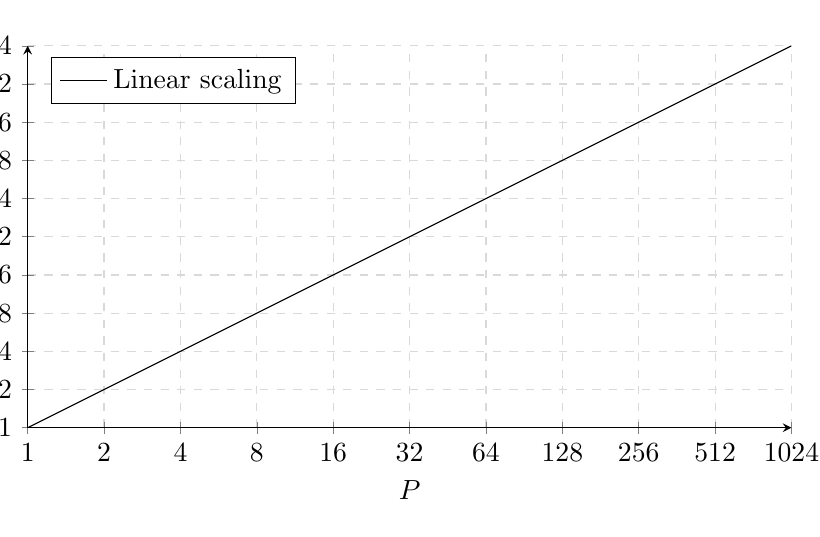
\begin{tikzpicture}[trim axis left, trim axis right]
\begin{axis}[
    % Set width to less than text width for equal margins
    width=0.8\textwidth,
    height=0.4\textwidth,
    scale only axis,
    xmode=log,
    ymode=log,
    log basis x=2,
    log basis y=2,
    domain = 1:1024,
    xmin=1,
    xmax=1024,
    ymin=1,
    ymax=1024,
    xtick={1,2,4,8,16,32,64,128,256,512,1024},
    xticklabels={1,2,4,8,16,32,64,128,256,512,1024},
    ytick={1,2,4,8,16,32,64,128,256,512,1024},
    yticklabels={1,2,4,8,16,32,64,128,256,512,1024},
    axis lines = left,
    xlabel = {$P$},
    ylabel = {Parallel speedup},
    xlabel style={font=\normalsize, below},
    ylabel style={font=\normalsize, above, rotate=0},
    tick label style={font=\normalsize},
    grid = major,
    grid style = {dashed, gray!30},
    domain = 1:1024,
    samples = 1000,
    smooth,
    no marks,
    legend pos = north west
]
\addplot [black] {x};
\legend{Linear scaling}
\end{axis}
\end{tikzpicture}
\caption{Strong scaling for the moment-based LBM code with slab decomposition.}
\label{fig:StrongScalingSlabDecomp}
\end{figure}%